\documentclass[brazil, a4paper,12pt]{article}
\usepackage[brazil]{babel}
\usepackage{graphicx}
\usepackage{geometry}
\usepackage[utf8]{inputenc}
\usepackage[T1]{fontenc}
\usepackage{url}
\usepackage{hyperref}
\usepackage{indentfirst}
\usepackage[usenames]{color}
\usepackage{ae,amsfonts,amsmath,amssymb,colortbl,keyval,lscape,paralist,
            xspace,setspace,subfigure,tabularx,times,listings,lettrine,
            pdftricks,textfit,titlesec,fancyhdr}
\geometry{a4paper,left=3cm,right=3cm,top=2.5cm,bottom=2.5cm}
\lstset{language=Java, tabsize=2, stringstyle=\ttfamily,basicstyle=\ttfamily, showstringspaces=false}

\begin{document}
\begin{titlepage}

  \vfill

  \begin{center}
    \begin{large}
      Universidade de São Paulo
    \end{large}
  \end{center}

  \begin{center}
    \begin{large}
      Instituto de Matemática e Estatística
    \end{large}
  \end{center}

  \begin{center}
    \begin{large}
      Programa de Pós-Graduação em Ciência da Computação
    \end{large}
  \end{center}

  \vfill

  \begin{center}
    \begin{Large}
        \textbf{MAC0431}\\
        \textbf{Introdução à Computação Paralela e Distribuída}\\
          Segundo Exercício Programa\\
    \end{Large}
  \end{center}

  \vfill

  \begin{center}
    \begin{large}
      Carlos Eduardo Moreira dos Santos\\
      Thiago Furtado de Mendonça
    \end{large}
  \end{center}

  \begin{center}
    \begin{large}
      Professor - Alfredo Goldman\\
    \end{large}
  \end{center}

  \vfill

  \begin{center}
    \begin{large}
      São Paulo \\
      \today \\
    \end{large}
  \end{center}

\clearpage
\tableofcontents 
\end{titlepage}

\section{Introdução}

Este trabalho visa analisar logs de servidores web e gerar dados para montar gráficos como o da Figura~\ref{fig:portal}. Ele mostra a média do tempo de resposta de um serviço conforme o número de clientes simultâneos aumenta. Um intervalo de confiança de 95\% também foi calculado para cada média, mas não é mostrado por ser muito pequeno neste caso.

A Figura~\ref{fig:portal} usou dados obtidos atráves de um gerador de carga sobre o serviço \emph{Portal} (a ser detalhado em \ref{sec:fmarket}). Além desse serviço, desejamos analisar o desempenho de todos os outros envolvidos na composição. Isso é possível através da análise dos logs de cada servidor, e o Hadoop nos ajudará a processar os 200 GB de logs do experimento executado.

\begin{figure}[!ht]
  \begin{center}
    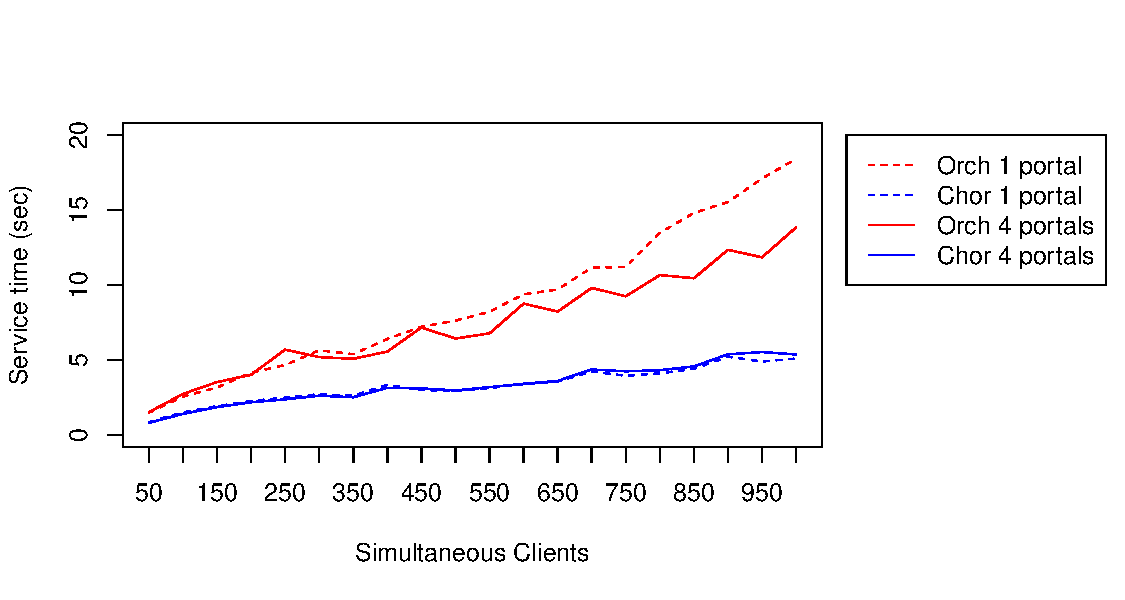
\includegraphics[width=\linewidth,clip=true,trim=1mm 6mm 3mm 20mm]{../talk/figures/portals1-4}
  \caption{Tempo médio de resposta do serviço \emph{Portal}.}
  \end{center}
  \label{fig:portal}
\end{figure}

\subsection{Caso de Uso}
\label{sec:fmarket}

O experimento utilizou a composição de serviços \href{http://github.com/choreos/future_market_choreography/}{Future Market}, escrita em java e implantanda em Apache Tomcat, sendo um serviço por máquina. Resumidamente, o gerador de carga simula um cliente que deseja comprar uma lista de produtos nos supermercados que oferecem o menor preço para cada um deles. Além dos supermercados, existem outros serviços como banco, fornecedor, fabricante, entrega de pacotes e registro de serviços.

Existem mais de uma instância de um determinado serviço, podendo haver até 17 no total em nosso experimento (em 17 servidores diferentes). Em particular, estamos interessados em comparar dois tipos de composição: orquestração e coreografia. No primeiro tipo, os serviços comunicam-se uns com os outros por intermédio do serviço \emph{Portal}, como podemos ver na Figura~\ref{fig:orch}. Já na coreografia, os serviços se comunicam diretamente, como na Figura~\ref{fig:chor}. 

\begin{figure}
  \begin{center}
    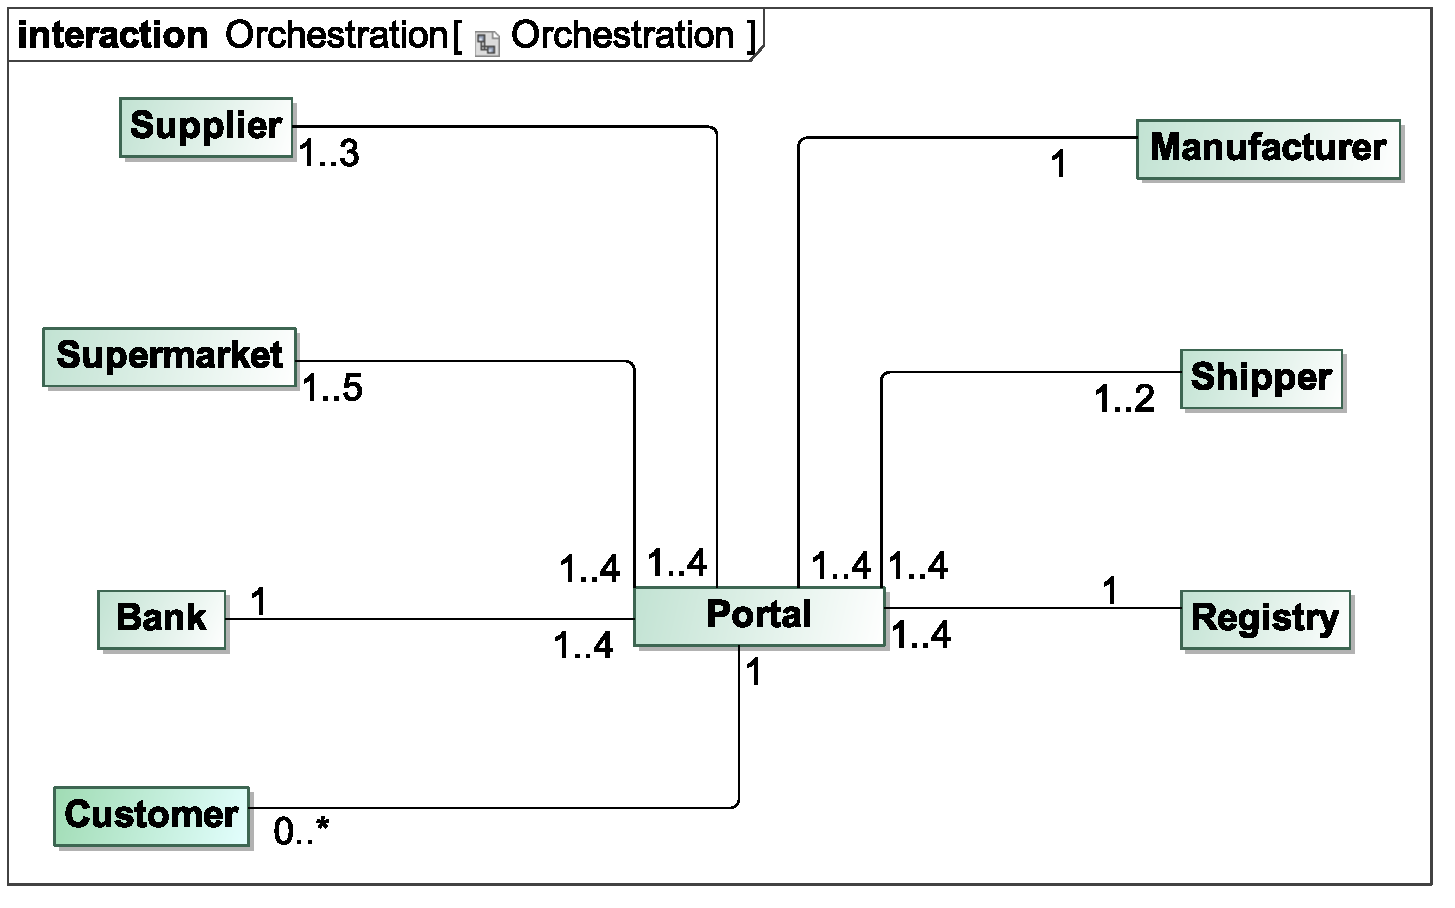
\includegraphics[width=\textwidth,clip=true,trim=7mm 9mm 8mm 16mm]{../talk/figures/orch}
    \caption{Interação entre serviços na versão com orquestração.}
    \label{fig:orch}
  \end{center}
\end{figure}

\begin{figure}
  \begin{center}
    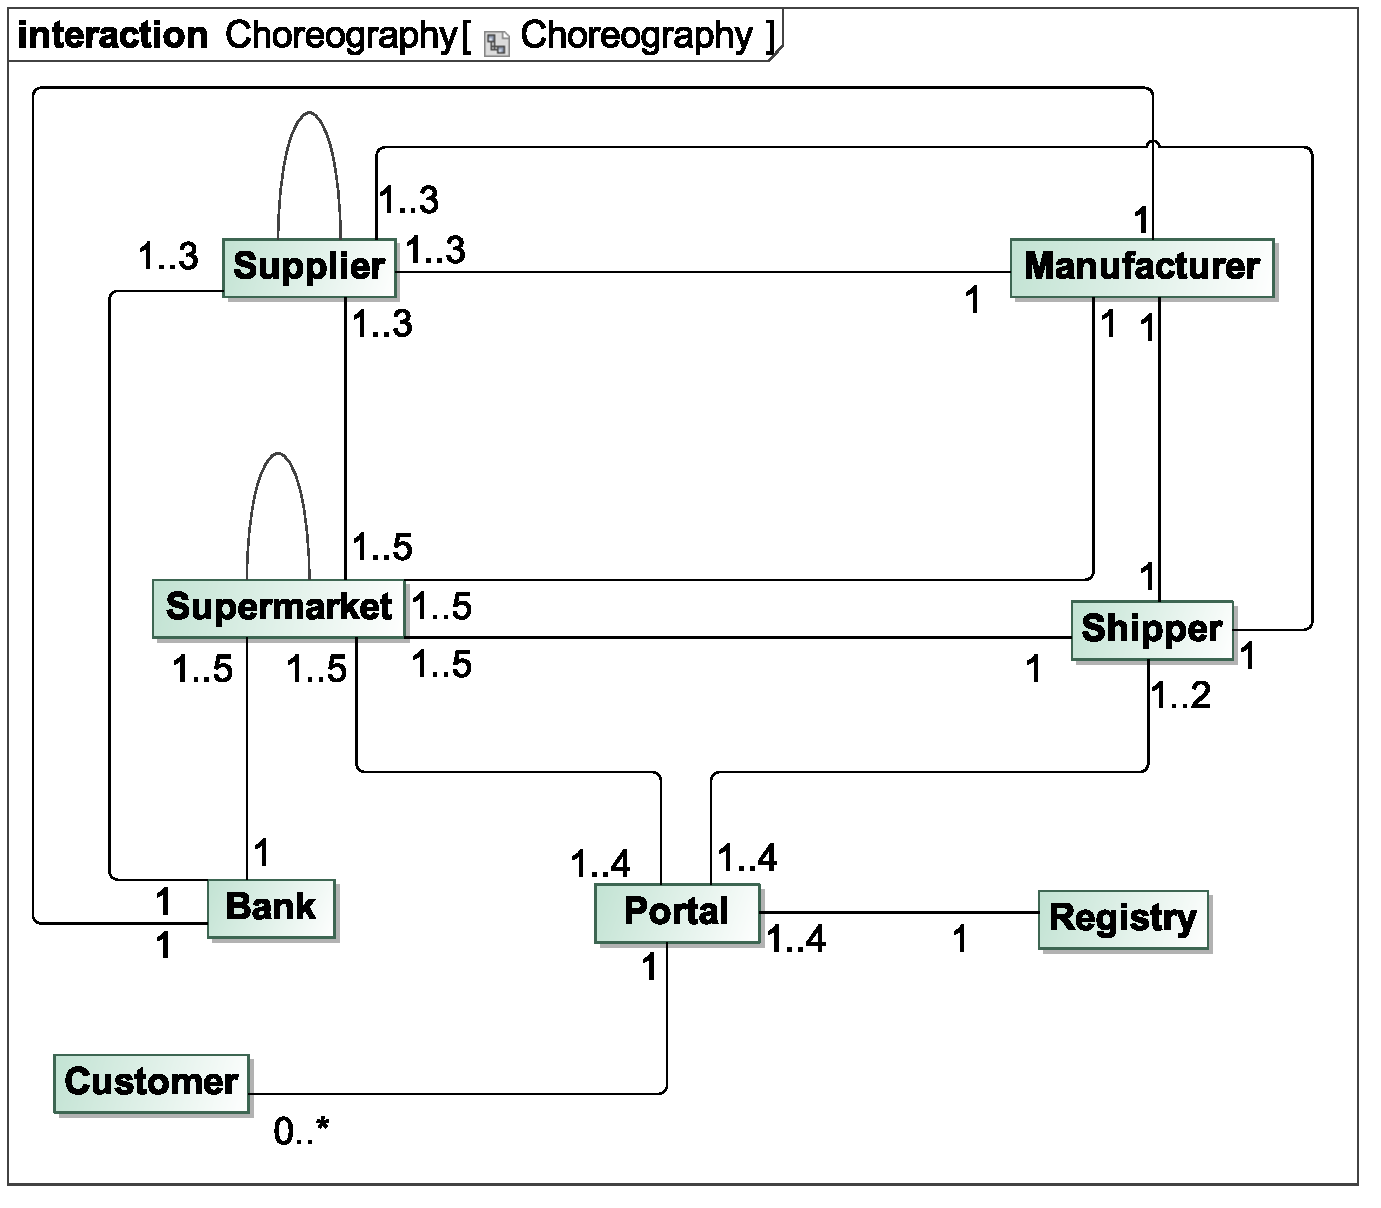
\includegraphics[width=\textwidth,clip=true,trim=2mm 10mm 5mm 14mm]{../talk/figures/chor}
    \caption{Interação entre serviços na versão com coreografia.}
    \label{fig:chor}
  \end{center}
\end{figure}

\section{Dados de Entrada}

\subsection{Gerador de Carga}
O gerador de carga desenvolvido para o \emph{Portal} produz um log no seguinte formato:

\begin{verbatim}
# orch,1,50,1349926295888
424
892
(...)
2017
2038
# orch,1,100,1349926297945
1110
1189
(...)
\end{verbatim}

As linhas que iniciam com \verb/#/ possuem a seguinte semântica:\\

\begin{tabular}{r l}
  {\bf orch,1} & Arquitetura (orquestração, {\bf1} portal)\\
  {\bf 50/100} & Número de clientes simultâneos (eixo x)\\
  {\bf 134552629...} & Instante da execução, em milissegundos
\end{tabular}
\\

Em seguida, os tempos de resposta são registrados um por linha, totalizando $n$ registros, onde $n$ é o número de clientes simultâneos. A simulação contém mais de uma ocorrência para uma dada arquitetura e número de clientes simultâneos.

\subsection{Log}
  O formato do log do Apache Tomcat foi modificado, possuindo um campo a mais que o padão no final, correspondente ao tempo de processamento da requisição. Como exemplo, temos a linha:

\begin{verbatim}
198.55.32.149 - - [09/Oct/2012:02:47:56 -0700] "POST
/supermarket5/orchestration HTTP/1.1" 200 914 811
\end{verbatim}

Neste exemplo, a requisição ao serviço \emph{Supermarket} de número 5 na orquestração demorou 811 milissegundos para ser processada. Note que não há como inferir, somente por esta linha, quantos clientes simultâneos estavam acessando o portal neste momento, assim como outras características da arquitetura (número de portais).

\section{Hadoop}

Utilizaremos MapReduce através do Apache Hadoop para calcular médias e desvios padrão por tipo de experimento num total de 200 GB de dados. Um tipo de experimento é determinado pelo tipo de composição, número de portais e pela quantidade de clientes simultâneos. Os códigos das funções \emph{Map} e \emph{Reduce} são apresentados nas próximas subseções.

\subsection{Map}

Nesta fase, geramos como chave o tipo de experimento e um identificador para o serviço (ex.: \emph{supermarket5}, \emph{bank}). Para tal, é necessário fazer a corespondência entre o tempo da requisição registrado no servidor web e o tipo de experimento em andamento no gerador de carga. Como exemplo, a função \\ \verb|getParams("10/Oct/2012:20:31:35")| retorna \verb/orch,1,50/. Caso o horário esteja fora do experimento, o retorno será vazio. Para o Map, o log do gerador de carga é interpretado e armazenado numa estrutura HashMap onde a chave é o \textit{timestamp} da requisição em milissegundos e o valor associado o tipo de experimento. Uma estrutura auxiliar é mantida em memória para que a análise possa ser feita levando em consideração que os experimentos estão ordenados em relação ao \textit{timestamp}.

A função \verb|getParams(long l)| recebe como parâmetro o \textit{timestamp} do log do Apache Tomcat e percorre as entradas do HashMap tentando associar a entrada do log do tomcat com uma das instâncias do experimento. Se \textit{t} é o parâmetro passado como valor de \verb/l/, então o retorno é o tipo de experimento que tem chave \textit{k}, \textit{ti <= k < tj}, para \textit{ti} e \textit{tj} duas chaves adjacentes, \textit{i < j}. 

A função \emph{Map}, para cada entrada, busca pelo experimento que fez a requisição e mapeia o tempo de resposta da requisição e é ilustrada pelo código a seguir:

\begin{figure} [!htb]
\begin{center}
\footnotesize
\begin{lstlisting}[numbers=left]
public void map(Object key, Text value, Context context)
		throws IOException, InterruptedException {

	if(!entryProcessor.matchesTomcatPattern(value.toString())) return;

	String[] itr = value.toString().split(" ");
	String timeString = itr[3].toString();
	Date date = entryProcessor.getDateInMillis(timeString.substring(1));

	if (date == null)
		return;

	String params = entryProcessor.getParams(date.getTime());
	if (!params.isEmpty()) {
		lineKey.set(itr[6].toString().concat("," + params));
		lineValue.set(Integer.parseInt(itr[itr.length - 1].toString()));
		context.write(lineKey, lineValue);
	}
}
\end{lstlisting}
\end{center}
\end{figure}

% Detailed explanation line by line of map funciton

\subsection{Reduce}
A função \emph{Reduce} receberá inúmeros tempos de resposta para cada tipo de experimento. Seu trabalho será o de resumir os dados em média e intervalo de confiança (necessário o cálculo do desvio padrão), como no pseudo-código abaixo:

\begin{figure} [!htb]
\begin{center}
\footnotesize
\begin{lstlisting} [numbers=left]
public void reduce(Text key, Iterable<IntWritable> values,
		Context context) throws IOException, InterruptedException {

	final Statistics stats = new Statistics();

	for (IntWritable value : values) {
		stats.addValue(value.get());
	}

	final double mean = stats.getMean();
	final double confInterval = stats.getCI();

	result.set("" + mean + "," + confInterval);
	context.write(key, result);
}
\end{lstlisting}
\end{center}
\end{figure}

\subsection {Dificuldades na implementação}

É importante notar que não é possível obter a quantidade de valores sem antes percorrer todo o iterador, nem reiniciá-lo após chegar no seu fim. Essas características dificultam o cálculo da média e do desvio padrão. Sem os devidos cuidados, a soma de $n$ elementos pode estourar o tipo primitivo. Além disso, o armazenamento de todos os valores para reutilizá-los pode exigir mais memória que o disponível.

\section {Conclusão}

\end{document}
